\documentclass[
    a4paper,
    12pt,
    bibliography = totoc,
    listof = totoc,
    listof = nochaptergap,
]{scrreprt}


% ================== Packages =================== %
\usepackage[utf8]{inputenc}
\usepackage{graphicx} % images
\usepackage{subcaption}
\graphicspath{ {./images/} }
\usepackage[top = 2.5 cm, bottom = 2.5 cm, left = 2.5cm, right = 2.5cm]{geometry}
\usepackage[T1]{fontenc} % correct encoding of european accent letters like ä, ö, ...
\usepackage{lmodern}
\usepackage{helvet}
\setkomafont{disposition}{\normalcolor\bfseries} % standard CM
\usepackage{amsmath}
\usepackage{float} % images
\usepackage{color}
\usepackage{abstract}
\usepackage[toc]{appendix}
\usepackage{makecell}
\usepackage{wrapfig}
\usepackage{caption}
\usepackage{amsmath}  % for \hookrightarrow
\usepackage{xcolor}   % for \textcolor
\usepackage[headsepline=0.75pt,footsepline=0.75pt]{scrlayer-scrpage}
\newcommand{\secref}[1]{\textit{\ref{#1} \nameref{#1}}} % custom citation
\addtokomafont{disposition}{\sffamily}
%\renewcommand*\sectfont{\sffamily\bfseries}
\usepackage{wrapfig} % Move tables and images
\usepackage[onehalfspacing]{setspace} % 1.5 spacing between lines
\usepackage{lipsum} % test page layout with lorem ipsum text
\usepackage[style=ieee, citestyle=numeric-comp, url=false]{biblatex}
\usepackage{tabularx}
\usepackage{enumitem, amssymb}
\usepackage{bm}
\usepackage{multirow}
\addbibresource{Literatur.bib}
\AtBeginDocument{\renewcommand{\bibname}{References}}
\usepackage[
    pdftitle = {214882-MasterThesis},
    pdfauthor = {Tobias Roth},
    hidelinks,
    citecolor = white
]{hyperref}

%=========== Checklist ==============%
\usepackage{pifont}
\newcommand{\cmark}{\ding{51}}%
\newcommand{\xmark}{\ding{55}}%
\newcommand{\done}{\rlap{$\square$}{\raisebox{2pt}{\large\hspace{1pt}\cmark}}%
\hspace{-2.5pt}}
\newcommand{\wontfix}{\rlap{$\square$}{\large\hspace{1pt}\xmark}}


% ============ Glossary ===============
\usepackage{acronym}

% =========== global document settings ===========
% do not indent paragraphs
\setlength{\parindent}{0pt} \setcounter{figure}{0}
\DeclareTOCStyleEntry[indent=0pt]{tocline}{figure}
\DeclareTOCStyleEntry[indent=0pt]{tocline}{table}

%========= Beginn des Dokuments ==========%

\begin{document}
\pagestyle{empty}
\pagenumbering{gobble}
\thispagestyle{empty}
~\\~\\
\begin{center}
    \begin{figure}
        \centering
        \begin{minipage}{.5\textwidth}
            \centering
            
\includegraphics[width=.8\linewidth]{frauenhofer.png}
        \end{minipage}%
        \begin{minipage}{.5\textwidth}
            \centering
            
\includegraphics[width=.8\linewidth]{hhn.png}
        \end{minipage}
    \end{figure}
    {\LARGE{Departement of Information Systems}\\\vspace*{0.3cm} Hochschule Heilbronn}
    ~\\ ~\\~\\

    {\large Master Thesis}\\
    ~\\~\\
  
    {\LARGE\textbf{Towards Quantum Graph Neural Networks for Molecular Property Prediction}}
    ~\\  ~\\ ~\\
    \small{submitted by}\\\vspace*{3mm}
    {\large\textbf{Tobias Roth}}\\
    ~\\ ~\\
    \today
    ~\\  ~\\ ~\\~\\
    \begin{tabular}{l c c l}
        First Supervisor            & & & Prof. Dr.-Ing. Carsten Lanquillon          \\
        Second Supervisor         & & & Prof. Dr.-Ing. Jochen Günther        \\
        Advisor & & & Philipp Wagner, M. Sc.   \\
    \end{tabular}
\end{center}
\thispagestyle{empty}
\chapter*{Eidesstattliche Erklärung}

\newlist{checklist}{itemize}{2}
\setlist[checklist]{label=$\square$}


Hiermit erkläre ich eidesstattlich, \\

1. dass die vorliegende Arbeit von mir selbstständig und ohne unerlaubte Hilfe angefertigt wurde, \\
2. dass ich alle Stellen (einschließlich Abbildungen und Tabellen), die wörtlich oder annähernd wörtlich oder dem Gedanken nach aus Veröffentlichungen und unveröffentlichten Unterlagen und Gesprächen entnommen worden sind, als solche an den entsprechenden Stellen innerhalb der Arbeit durch Zitate bzw. Verweise kenntlich und nachvollziehbar gemacht habe, einschließlich der Kenntlichmachung KI- generierter Texte oder Abbildungen, \\
3. die Arbeit noch bei keiner anderen Prüfung vorgelegt wurde. \\
Zum Einsatz von KI-basierten Instrumenten (wie z.B. ChatGPT) erkläre ich, dass für die vorliegende Arbeit 
    
\begin{checklist}
    \item[\wontfix] kein Einsatz erfolgte
    \item ein Einsatz in folgender Form erfolgte:
\end{checklist} 

Ich bin mir  bewusst, dass eine falsche Erklärung rechtliche Folgen haben wird. Insbesondere ist mir bewusst, dass eine Note auch nach der Veröffentlichung angepasst werden kann, wenn die Täuschung erst zu einem späteren Zeitpunkt bekannt geworden ist, z.B. durch fortgeschrittene Prüfprogramme. Die nachträgliche Anpassung kann auch noch nach Abschluss des Studiums erfolgen. In diesem Fall wird das unrichtige Zeugnis (inkl. Urkunde und  Diploma Supplement) eingezogen.

{\raggedright
\vspace{2.5cm}

\hrulefill \hspace{1cm} \hrulefill \hspace{1cm} \hrulefill \\ 

\textit{Ort, Datum \hspace{3.25cm} Name, Vorname \hspace{2.6cm} Unterschrift}}
%\include{Danksagung.tex}
%\renewcommand{\abstractname}{Abstract}
\begin{abstract}
    
\end{abstract}

%============ Verzeichnisse =================%
\cfoot{\pagemark}
\pagenumbering{Roman}
{\sffamily\tableofcontents}
\addchap{List of Abbreviations}
\begin{acronym}[TestTestTestTest]\itemsep=-3pt
    \acro{CRISP-DM}[CRISP-DM]{Cross Industry Standard Process for Data Mining}    
    \acro{GAE}[GAE]{Graph Auto Encoder}
    \acro{GAN}[GAN]{Graph Attention Network}
    \acro{GCN}[GCN]{Graph Convolutional Neural Network}
    \acro{GNN}[GNN]{Graph Neural Network}
    \acro{GIN}[GIN]{Graph Isomorphism Networks}
    \acro{GraphSAGE}[GraphSAGE]{Graph Sample and Aggregated}
    \acro{GraphSNN}[GraphSNN]{Graph Symmetric Neural Network}
    \acro{MPNN}[MPNN]{Message Passing Neural Network}
    \acro{PES}[PES]{Potential Energy Surface}
    \acro{RecGNN}[RecGNN]{Recurrent Graph Neural Network}
    \acro{STGNN}[STGNN]{Spatial-temporal Graph Neural Networks}
    \acro{QGNN}[QCNN]{Quantum Convolutional Neural Network}
    \acro{QGNN}[QGCN]{Quantum Graph Convolutional Neural Network}
    \acro{QGNN}[QGNN]{Quantum Graph Neural Network}
    \acro{QGNN}[QGRNN]{Quantum Graph Recurrent Neural Network}
    \acro{QML}[QML]{Quantum Machine Learning}
    \acro{Qubits}[Qubits]{Quantum Bits}

\end{acronym}
{\sffamily\listoffigures}
{\sffamily\listoftables}
\newpage

%============ Contents ===================%
\pagestyle{scrheadings}
\renewcommand\chapterpagestyle{scrheadings}
\automark[chapter]{chapter}
\chead{\rightmark}
\cfoot{\pagemark}
\pagenumbering{arabic}
\chapter{Global Introduction}
\label{chap:Introduction}
\section{Problem Definition}
\label{sec:problemdefinition}
In view of the steadily advancing climate change, efforts to reduce environmental pollution are
increasingly coming into focus both in the public eye and within the scientific community \cite{amin_hydrogen_2022}.
This includes the search for scalable and cost-effective renewable energy storage solutions, which
is essential to meet the world's growing energy demand while mitigating climate change \cite{kilkis_research_2019}. The
conversion of electricity to hydrogen, as well as the reverse combustion process, can play an
important role here \cite{amin_hydrogen_2022}. Therefore, new materials are constantly being investigated to enable
catalytic processes in the field of hydrogen production to run efficiently \cite{chen_waste-derived_2023}. Machine learning
methods are already being used to simulate and calculate catalytic properties. In particular, graph
neural networks (GNN) are proving to be especially promising here \cite{tran_open_2023, bronstein2017geometric}. Since the prediction of
potential areas and other relevant properties proceeds at the molecular and atomic level, the use
of quantum computers is also being investigated. In the literature, first approaches to realize
GNNs on quantum computers already exist \cite{verdon_quantum_2019,beer_quantum_2021,ai_decompositional_2023}.

\section{Aim of this work}
\label{sec:aim}
This master’s thesis investigates the extent to which quantum GNNs are suitable for predicting
molecular properties. To achieve this, the first step is to acquire an understanding of GNNs and
the foundations of quantum computing, which will be discussed in this work. Subsequently, a
classical GNN will be implemented to predict molecular properties using available data. Later in
this thesis, a quantum GNN will be designed and developed that uses the same input data as the
classical GNN. The quantum GNN will be tested and evaluated on a quantum computer. Having a classical and a quantum GNN, a comparison of performance between these models will take place.

\section{Global Research Questions}
\label{sec:RQs}
In order to solve the presented problem, the following research question and sub-questions are created: \\
\textit{How can classical and quantum graph neural networks be used for the prediction of molecular properties?}  \\~\\
Q1: How do GNNs and quantum GNNs work? \\
Q2: How must molecular data be processed to be used with a quantum computer? \\
Q3: Are quantum GNNs suitable for predicting molecular properties in the context of electrocatalysis?\\
Q4: How does the performance compare to classical GNNs?

\section{Global Research Methodology}
\label{sec:RM}
For the scientific design of the research process, this work will follow the established procedure according to Peffers et al. \cite{peffers_design_2007}, as illustrated in Figure \ref{img:generalRM}. Based on this, the research process is structured into different steps, which are explained below. 

\begin{figure}[h]
\centering
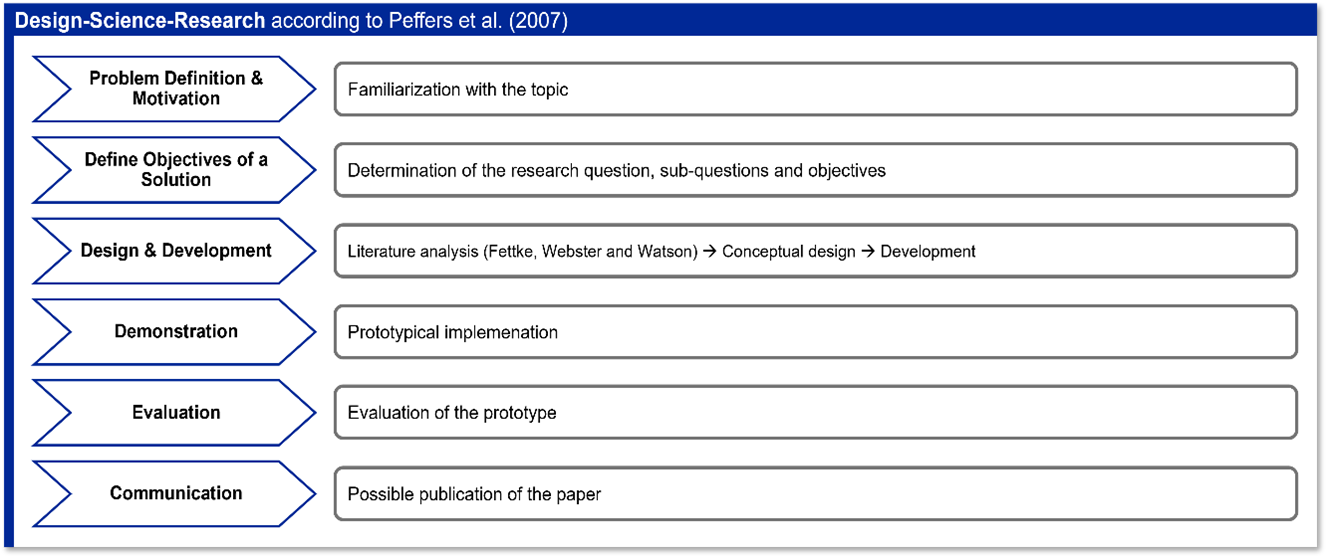
\includegraphics[width=\textwidth]{01_generalRM.png}
\caption[Overview of the general research methodology]{\label{img:generalRM}{Overview of the general research methodology \cite{peffers_design_2007}}}    
\end{figure} 

Previously, the problem upon which this work is based on and the objectives to be achieved within this work were defined in cooperation with the Frauenhofer IPA. \\

In the next steps, a comprehensive and structured literature review will be conducted with the aim of identifying the necessary foundations for GNNs, quantum computing, and the relevant molecular properties. The literature review will follow the methods of Fettke \cite{fettke_state---art_2006}, Webster and Watson \cite{webster_analyzing_2002}, as well as vom Brocke et al. \cite{vom_brocke_reconstructing_nodate}. Relevant literature databases and other elements
will be defined at the time of conducting the literature review. The results of the literature review form the first part of this work and will be documented in the form of a state-of-the-art paper.
Afterwards a classical GNN will be designed and developed to predict molecular properties using the existing data set. This serves to establish a basic understanding of GNNs and the dataset as well as possible results of the prediction. Furthermore, the classical GNN will be utilized to compare its results and performance with the quantum GNN, including various performance metrics such as accuracy.
After the successful implementation of the classical GNN, a quantum GNN will be designed and developed, which is the core focus of this thesis. The development of a quantum GNN involves using different tools and frameworks compared to a classical GNN, including the preprocessing of the available dataset. This prototype will undergo testing, evaluation, and potential optimization using a quantum computer. Specific requirements for the GNN and potential evaluation criteria will be defined as part of the research process. This can be achieved through the conducted literature review or other methods, such as expert interviews. With both classical and quantum GNNs in place, an extensive comparison between these models will be conducted. The results of this procedure constitute the second part of this thesis. The entire process and its findings will be documented.

\chapter{Paper 1 - Architectures of Graph Neural Networks}

\section*{Abstract}

As deep learning algorithms increasingly adress graph-structured data, Graph Neural Networks (GNNs) play a more and more important role in various fields, including computational chemistry and the prediction of molecular properties. However, currently in the literature different architectures and approaches of GNNs exist. Therefore, this paper analyzes the current state-of-art by exploring architectures and approaches of GNNs in the literature. By creating an overview, it will show that convolutional GNNs are commonly used and particulary reliable when working with molecular properties. With the help of structured process CRISP-DM, later a convolutional GNN will be developed that predicts the potential energy surface of molecules with the QM9 dataset and a simpler water dataset. The evaluation shows a high level of accuracy compared to a classic neural network architecture, especially for more complex datasets. Therefore, the GNN was succesfully developed. \\


\textit{\textbf{Keywords:} graph neural networks, architectures, literature review, potential energy surface prediction}

\section{Introduction}
While deep learning algorithms effectively capture hidden patterns of Euclidean data, there is an increasing number of application areas where the data is represented in the form of graphs or structures similar to graphs \cite{wu_comprehensive_2021}. Due to the expressive capabilities of graphs, researches on analyzing these kind of structures with machine learning have been receiving more and more attention. This is evident in the areas of social science, such as social networks, natural science like physical systems, knowledge graphs and other research areas \cite{zhou_graph_2020}. Deep learning based methods that operate in a graph domains are called Graph Neural Networks (GNNs) \cite{velickovic_everything_2023}. \\ 
In computational chemistry, molecules are modeled as graphs enabling various experiments \cite{wu_comprehensive_2021}. This includes the prediction of potential energy surfaces for  molecules made of hydrogen compounds or other materials \cite{liu_computational_2023}. In the current literature, different approaches or architectures for GNNs exist \cite{wu_comprehensive_2021}. This raises the question of which approaches are available and which of these approaches is well suited for the prediction of molecular properties such as potential energy surfaces. \\

In order to solve the presented problem, the following research question and sub-questions are created: 
\begin{center}
    \textit{"How can a Graph Neural Network for the prediction of molecular properties be developed?"} \\
\end{center}
Q1: \textit{What approaches for Graph Neural Networks currently exist in the Literature?} \\
Q2: \textit{What architecture suits the prediction of molecular properties best?} \\

The goal of this paper is to develop an understanding of graph neural networks in general and the different types of architectures that exist in the literature. Besides, in the scope of this thesis, an understanding of the prediction of potential energy is created. Based on this procedure, the literature review will show what architecture of graph neural networks suits the prediction of potential energy best. In summary, to answer the developed research question and sub-questions, the following artifacts will be created as part of the research: 

\begin{itemize}
    \item literature review of different graph neural network architectures
    \item prototypical implementation of a graph neural network for the potential energy 
    prediction
    \item baseline neural networks for the comparison to graph-based models with different datasets
\end{itemize}  

The structure of this paper is as followed: first, the scientific foundations and theoretical background are discussed. Then the research methodology is presented in detail. Based on this, the findings and their results are presented and then discussed. Finally, a conclusion and discussion of the results is provided, as well as an overview of possible research topics based on this work.  

\section{Theoretical Background}
\subsection{Graph Neural Networks}

Graph Neural Networks (GNNs) are a type of neural networks that are used to work with graph-structured data. They provide a framework for tasks that focus on learning dependencies and interactions between data points. GNNs use the structure of graphs to capture and process information in way that is not possible using traditional neural networks \cite{duvenaud2015convolutional}. In the context of GNNs a graph consists of nodes that represent entities and edges that describe relationships between those entities. The objective of GNNs is to learn important node representations that contain both local and global graph information. \cite{wu_comprehensive_2021} GNNs are effective in dealing with non-Euclidean and irregular data structures. This makes GNNs very suitable for domains where relationships between data points are as important as, or even more important then, the individual data points itself \cite{zhou_graph_2020}. \\

The architecture of a GNN consists of layers that update node representations by aggregating information from neighboring nodes iteratively. This process enables nodes to relearn their understanding of the local context while considering the wider structure of the graph. The aggregation step involves weighted summation or concatenation of features from neighboring nodes, allowing each node to summarize information from its surroundings. \cite{velickovic_everything_2023, xu_how_2019} A key aspect of a GNN is the neighborhood aggregation function, which is also known as the message-passing mechanism \cite{gasteiger_directional_2022}. This function defines how information between nodes in each layer is exchanged. The power of GNNs lies in their ability to progressively enhance node representations through multiple layers, capturing detailed dependencies within the graph. 

\subsection{Potential Energy Surface Prediction}
The potential energy surface (PES), in the context of molecules and atoms, describes the energy of a molecule in regard to certain parameters, e.g. to the position of its atoms.    
Predicting the potential energy surface of atoms is a task in computational chemistry and materials science. It gives information about the stability and properties of molecules and materials \cite{liu_computational_2023}. This is helpful when to decide whether materials can be used to enable efficient catalytic processes in the field of hydrogen production \cite{chen_waste-derived_2023}. 

\section{Research Methodology}
First, the given problem of the prediction of molecular properties with GNNs was investigated. For this purpose, an initial investigation of the literature took place and the topic was explored. This is followed by the definitions of the research questions as well as the sub-questions and the delineation of the research topic. \\

\begin{figure}[h]
    \centering
    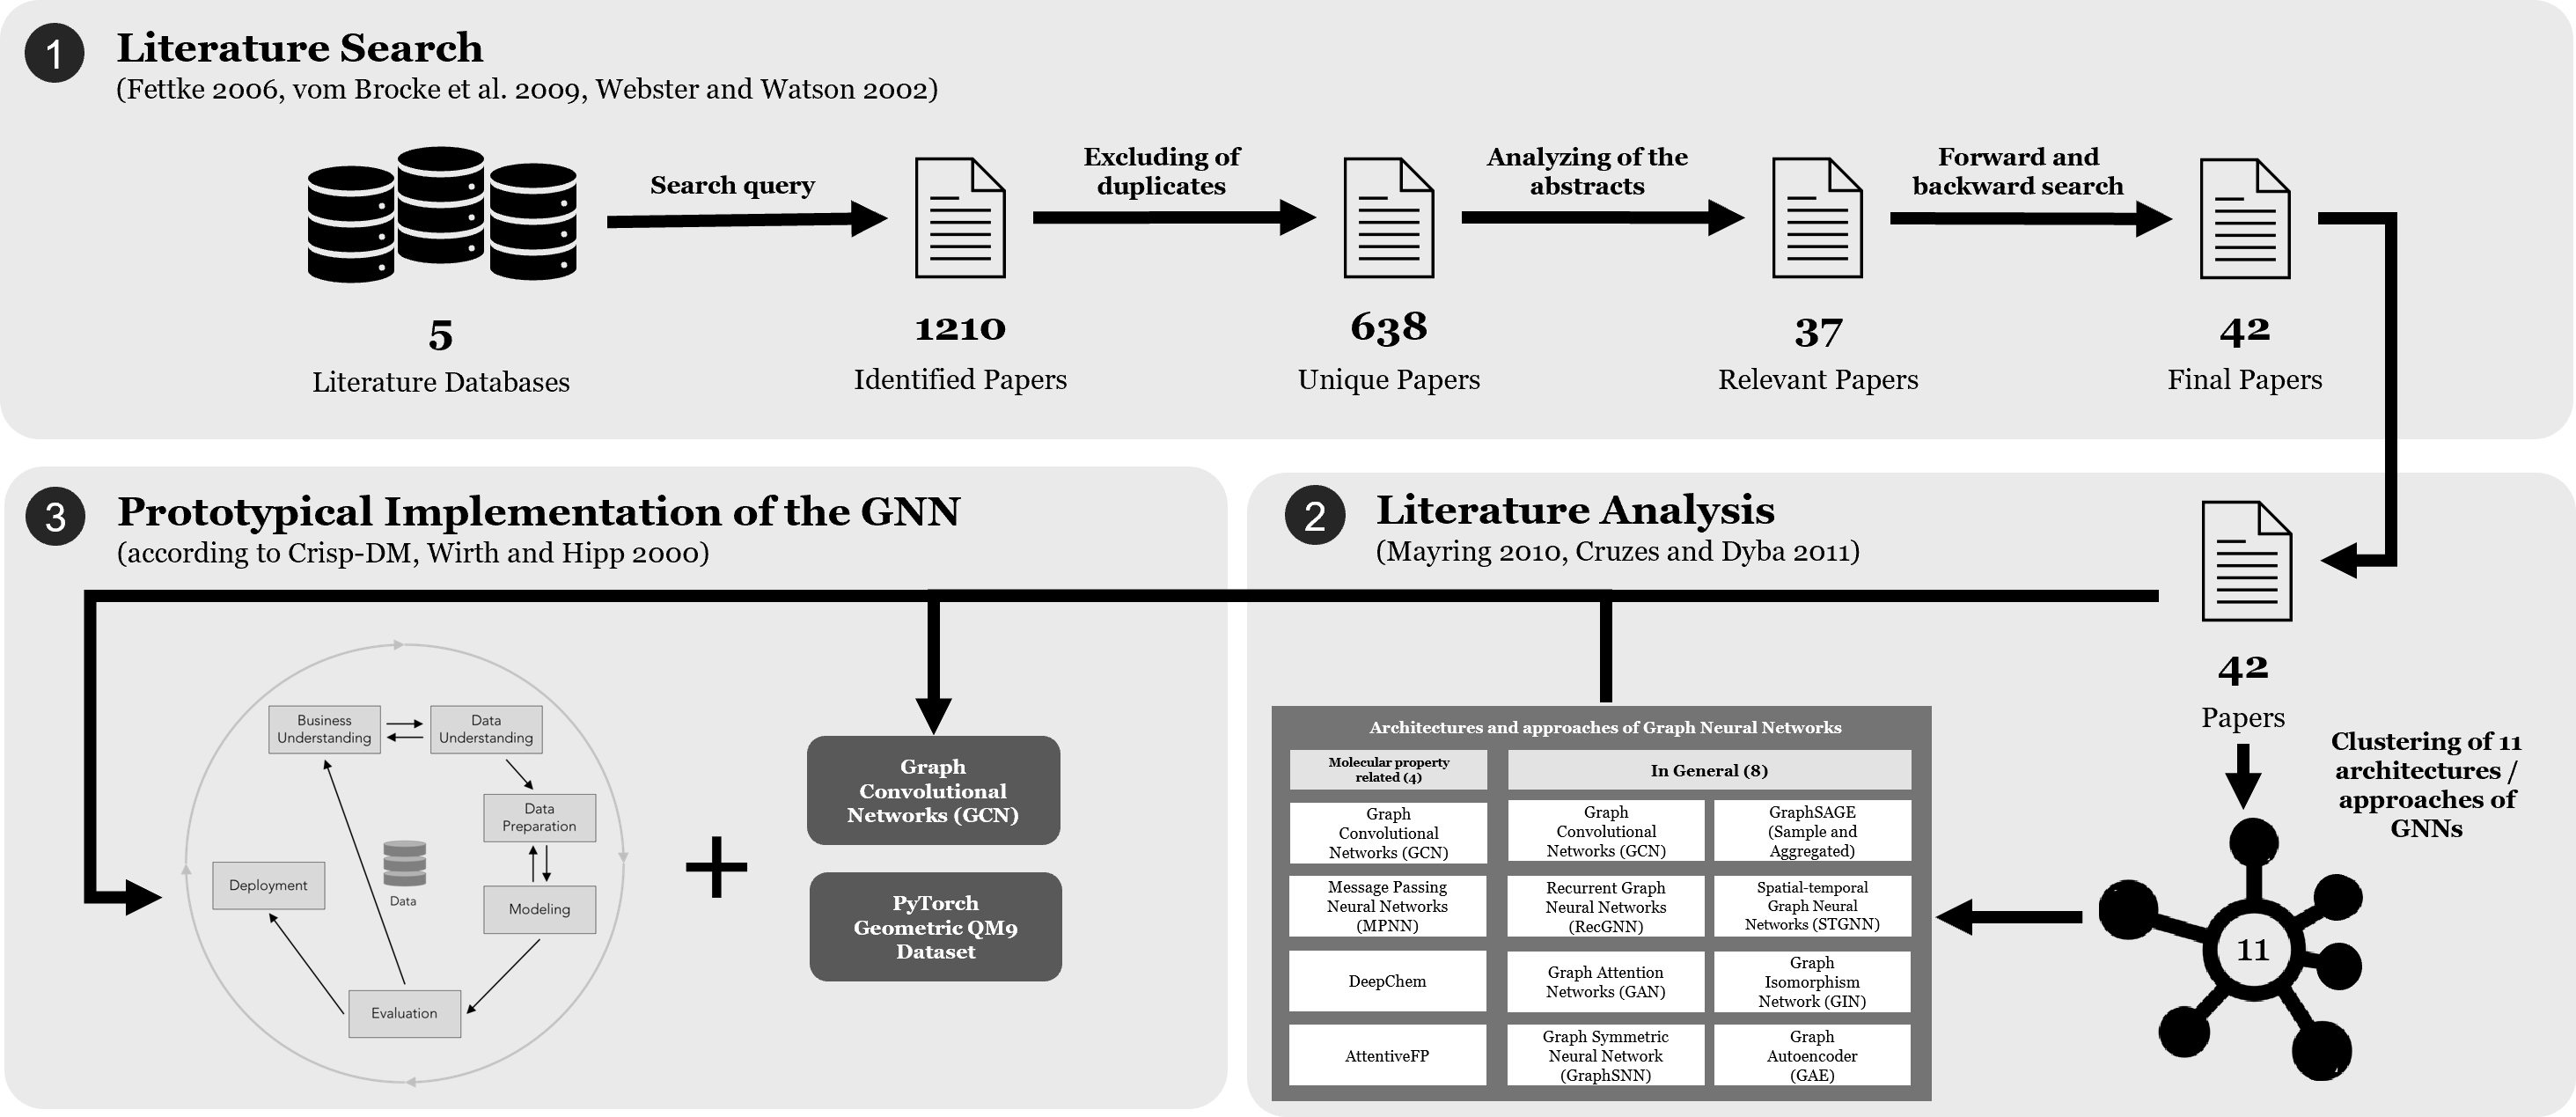
\includegraphics[width=0.95\textwidth]{02_paper01RM.png}
    \caption[Overview of the conducted research process]{\label{img:paper01rm}{Overview of the conducted research process}}
    \end{figure} 

Afterwards, a comprehensive and structured literature review is conducted with the aim of identifying different approaches of GNNs and finding the most suitable for molecular property prediction. The findings of this literature review are used for the creation of a common understanding of GNNs in the given context. In the next step, a GNN is prototypically implemented with the available dataset. This serves the goal of being able to directly test and evaluate the developed GNN. For better structuring and traceability of the procedure, the exact research process is shown in Figure \ref{img:paper01rm}, which is also described in detail in the following section. \\

In the \textbf{first step}, the literature search based on Fettke \cite{fettke_state---art_2006}, vom Brocke et al. \cite{vom_brocke_reconstructing_nodate} and Webster and Watson \cite{webster_analyzing_2002} was performed. The following literature databases were used: IEEE Xplore Digital Library, ScienceDirect, SpringerLink, Emeralt Insight and Google Scholar. Electronic searches of titles using the search terms [("Graph Neural Networks") AND (("architectures") OR ("approaches"))] and [("Graph Neural Networks") AND ("*molecular*")]. Moreover, no specific period of time was selected. According to the search query performed, these searches resulted in a total of 1210 publications. After analyzing abstract and keywords, 37 relevant publications remained for the given research focus. In addition to the database search, Webster and Watson \cite{webster_analyzing_2002} recommend performing a forward and backward search. These were performed in a final step and increased the number of final publications to 42. \\

In the \textbf{second step}, a total number of 42 papers were read in full and coded. For the clustering of the architectures and approaches of GNNs the procedure of Fettke \cite{fettke_state---art_2006} was performed. After this process of clustering, a total of 11 different architectures and approaches for GNNs could be identified. According to the research topic, this results are assigned into two different higher-level categories, "molecular property related" and "In General". \\

The \textbf{third step} covers the prototypical implementation of the GNN for molecular property prediction. Based on the findings of the literature review, a GNN is implemented and evaluated that predicts potential energy surfaces with the QM9 Dataset from Pytorch Geometric \cite{noauthor_torch_geometricdatasetsqm9_nodate}. The implementation of the GNN follows the established procedure of CRISP-DM \cite{wirth2000crisp} and is explained later in this paper. 

\section{Findings}
In this section, the results and findings are presented and discussed in detail. Especially the literature review and the prototypical implementation of the GNN for the prediction of potential energy will be considered. 


\subsection{Literature Review}

After the conduction of the literature review, two categories of GNN architectures and approaches could be identified, namely "molecular property related" and "In General". The first category lists all GNN architectures that are applied in computational chemistry, especially in working with molecular properties. The second category "In General"  describes general GNN architectures that occur in literature and also for other application areas. For both categories, different architectures and approaches were found, which are shown in Figure \ref{img:paper01findings}. In the following, the findings will be explained in more detail.

\begin{figure}[h]
    \centering
    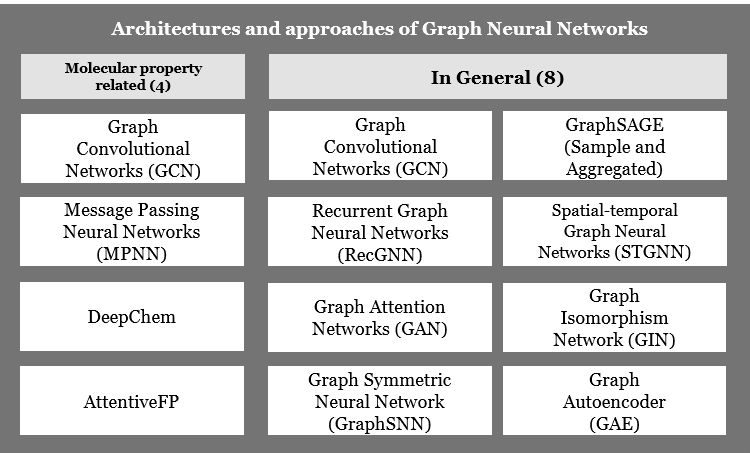
\includegraphics[width=0.95\textwidth]{03_lr_ergebnisse.png}
    \caption[Overview over die identified architectures and approaches for GNNs]{\label{img:paper01findings}{Overview over die identified architectures and approaches for GNNs}}
\end{figure} 

For the processing of data related to molecular property or computational chemistry, in the literature for different types of GNN approaches could be identified: Graph Convolutional Networks (GCN), Message Passing Neural Networks (MPNN), DeepChem and AttentiveFP. \\

Proposed by Gilmer et al. in 2020 \cite{gilmer_neural_2017}, Message Passing Neural Networks (MPNNs) are a class of graph neural networks designed for processing graph-structured data, targeting the application areas of chemistry and molecular property prediction. The architecture of MPNNs consists of message passing, updating node and edge representations iteratively through message passing functions, enabling the model to capture relationships reliable within the graph. The key components include message passing, aggregation, and readout. During message passing, information from neighboring nodes and edges is aggregated and transformed through learnable functions. Aggregation mechanisms, often involving summation or attention, allow nodes to incorporate information from their local environments. A readout function then processes the final node representations to make predictions about the entire graph. This design enables MPNNs to effectively handle variable-sized graphs and adapt to diverse molecular structures. \\

Unlike the other findings, DeepChem is no GNN itself, but a Python library for machine learning and deep learning on molecular and quantum datasets. The library consists of a extensive toolkit for working with molecular property prediction and related tasks \cite{noauthor_deepchem_nodate}. For example, DeepChem offers different deep learning models, including graph convolutional networks, graph attention networks, and recurrent neural networks. DeepChem is used for research in the field of computational chemistry and drug discovery \cite{altae-tran_low_2017}. \\

AttentiveFP is a deep learning model for graph data, which integrates attention mechanisms into GNNs.  In the area of computational chemistry, AttentiveFP captures and values the importance of specific atoms in a molecule. This model gives attention weights to highlight relevant atoms during information aggregation. In this way, the model is able to focus on specific regions within a molecular graph. The architecture of AttentiveFP involves message-passing steps where atoms exchange information based on their local environments. The attention mechanism assigns an importance scores to neighboring atoms, enabling the model to prioritize interactions between them. The focus on local context is particularly beneficial when handling various molecular structures. The attention-based approach enhances the capacity to recognize subtle chemical patterns, making it useful for applications in computational chemistry. According to its architecture, AttentiveFP is a specific Graph Attention Network (GAN). \cite{xiong_pushing_2019,jiang_could_2021} \\

The literature review showed that Convolutional Graph Neural Networks (GCNs) are both used for working in the field of molecular property prediction and in other application areas. Introduced by Kipf and Welling in 2016 \cite{kipf2016semi} GCNs are one of the earliest and commonly used architectures of GNNs \cite{wu_comprehensive_2021}. 

\begin{figure}[h]
    \centering
    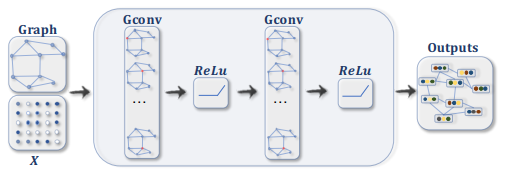
\includegraphics[width=0.95\textwidth]{04-convgnn.png}
    \caption[Examplary GCN architecture for node classification]{\label{img:paper01gcn}{Examplary GCN architecture for node classification \cite{wu_comprehensive_2021}}}
\end{figure} 

GCNs enable the modeling of molecular structures by learning node representations through a certain amount of graph convolutional layers. These layers aggregate information from neighboring atoms, allowing the model to learn relationships within graph data. The main point of the functionality of a GCN is the ability to weight these aggregations, highlighting more important atoms and interactions. \cite{zhang2019graph} Figure \ref{img:paper01gcn} shows an examplary architecture for a GCN: graph data is used as input, the GCN consists of two convolutional layers where ReLu is used as activation function and the output is a predicted property of the input data. \\
The architecture of GCNs involves iterative information propagation through the graph. Each layer computes a weighted sum of neighboring node features, producing node representations. The weight parameters are learned during the training of the model, allowing the GCN to adapt to the characteristics of the respective graph dataset. GCNs are especially effective when working with molecular structures, because the hierarchical structure of a GCN enables the learning of global information, which is required for having a holistic understanding of molecular structures and perform tasks effectively. \cite{wu_comprehensive_2021, zhang2019graph} \\

For the general use of GNNs and other application fields, a total of eight different approaches of GNNs could be identified: the previously explained GCNs, GraphSAGE (Sample and Aggregated), Recurrent Graph Neural Networks (RecGNN), Spatial-temporal Graph Neural Networks (STGNN), Graph Attention Networks (GAN), Graph Isomorphism Networks (GIN), Graph Symmetric Neural Network (GraphSNN),  and Graph Autoencoder (GAE). While AttentiveFP is a specific GAN, the structure and functionality of GANs is similar to that of AttentiveFP described above \cite{xiong_pushing_2019}. For reasons of focus, only the RecGNNs and GAEs are discussed below. \\

Recurrent Graph Neural Networks (RecGNNs) extend the possibilities of traditional GNNs by using both graph-based and recurrent components. Thereby, temporal information and sequential patterns within graphs can be captured. At each time step, the model updates node representations using graph convolutional layers and captures the structure of the evolving graph. Simultaneously, recurrent units capture a memory of past states, which enables the model to save information for a certain time step. The recurrent nature of RecGNNs allows them to learn and represent evolving graph structures. This is especially helpful for a dataset where the relationships between the data show temporal dynamics, e.g. in time-sensitive domains. \cite{li2017diffusion,hajiramezanali2019variational} \\

Designed for learning representations of graph-structured data, Graph Autoencoders are neural network models that are a tool especially helpful for the reconstruction of nodes and graphs. GAEs encode graph-structured input into low-dimensional vectors. By doing so, the essential structural features are captured while the graph typology is preserved. This approach is to be classified as unsupervised learning and supports GAEs in applications like link prediction or anomaly detection. The architecture of GAEs consist of an encoder and a decoder. The encoder maps nodes or graphs to lower-dimensional representations, while the decoder reconstructs the original input from the previously created embeddings. Similar to other variants of GNNs like the RecGNNs, GAEs leverage graph convolutional layers to aggregate information from neighboring nodes during encoding, facilitating the learning of meaningful representations. \cite{li2021adaptive, zhang2021graph}

\subsection{Development of the GNN}
After gaining insight into different architectures and approaches of GNNs in the literature, in the following the development of the GNN for the prediction of potential energy surfaces will be explained. In the course of this paper, a GCN is developed and used with the QM9 Dataset \cite{noauthor_torch_geometricdatasetsqm9_nodate}. In addition, the developed model was trained a second time using a data set containing only water molecules. This will be used to compare the performance of different data sets on the models. The development of the GCN was based on the established CRISP-DM process \cite{wirth2000crisp}, which is explained step by step below. \\

In the initial Phase, the Business Understanding, the goal is to understand the research objectives and requirements. In view of the advancing climate change, the reduction environmental pollution plays an important role for humankind \cite{amin_hydrogen_2022}. This includes the search for scalable and cost-effective renewable energy storage solutions, e.g. like the conversion of electricity to hydrogen as well as the reverse combustion process \cite{kilkis_research_2019}. For this purpose, new materials are being investigated, to enable efficient catalytic processes in the field of hydrogen production \cite{chen_waste-derived_2023}. Machine Learning Methods, like GNNs, are used to simulate and calculate catalytic properties like the prediction of potential energy surfaces \cite{tran_open_2023}. Therefore, the goal of the developed GNN in this paper is to predict the potential energy surfaces of different molecules. \\

The focus of the second step, namely Data Understanding, is to gain insight into the given dataset. The QM9 Dataset consists of approximately 130,000 molecules with 19 regression targets \cite{noauthor_torch_geometricdatasetsqm9_nodate}. 
Within all the different molecules, there are five potential atom types like Carbon and Oxygen and four different types of chemical bonds between them (single bond, double bond, etc.) \cite{menonunderstanding}. For the usage of the GNN, the molecules are transformed, whereas the atoms form the nodes of the graph and the edges are described through the chemical bonds between the atoms. The relevant regression target for the prediction of potential energy surface is the seventh target of the QM9 Dataset, the Internal energy at 0K. The water dataset contains only water molecules with oxygen and hydrogen atoms. In summary, there are approximately 36,000 water molecules in this dataset with different atomic positions or coordinates. Therefore, compared to the QM9 dataset, the water dataset is not as complex in terms of the number of different atoms and chemical bonds and also in the general size of the dataset. The water data set is also used to predict the potential energy surface. \\

In the third step, the available data will be prepared to be able to train the developed GCN. The data preparation includes at first the extraction of all relevant information from the dataset, which is in this case the atoms, the cartesian coordinates, and the Internal energy at 0K. For better results of with the model prediction, the target variables are normalized with the help of their mean and standard deviation. Another important step in the data preparation is the conversion of the coordinates into inverse pairwise distance, so that the GCN understands the spatial relationships like translation and rotation invariance between the atoms in the molecular structure. The same procedure goes for the water dataset.\\

After the data preparation, the GNN architecture is implemented during the modeling phase of the CRISP-DM process. The GNN consists of two convolutional layers, with the before prepared nodes, edges and features as well as the initialized weights as input parameters. The activation function is LeakyRelu. The neural network is implemented with the PyTorch Python package. Before the training, the dataset is randomly split into training and validation dataset, for the evaluation of the model in the next step.\\

The fifth phase describes the evaluation of the developed model, where the performance of the model is assessed with the validation dataset. With the help of the Adam optimizer algorithm, also implemented in PyTorch, the model is optimized during training. With this procedure, the ability of the model to generalize and make accurate prediction on data other than the training data is enhanced. Since the prediction of the potential energy surfaces is a regression task, the performance of the model can be measured by using different regression performance metrics. The following performance metrics are used: Model Training Time (lower is better), Mean Squared Error (lower is better), Root Mean Squared Error (lower is better) and the $R^2$-Score (higher is better). In the following, the performance metrics are evaluated by comparing the performance of a baseline (non-graph-based) neural network architecture with the implemented GCN architecture, where the different approaches are trained individually for each dataset. Table \ref{tab:paper01performancecomparisonqm9} lists the computed metrics for the training with the QM9 dataset.

\begin{table}[h!]
    \centering
    \captionsetup{justification=centering}
    \resizebox{\textwidth}{!}{
        \setlength{\tabcolsep}{1.5em}
        {\renewcommand{\arraystretch}{1.5}% for the vertical padding
            \begin{tabular}{p{7cm} l l}
                \hline
                 \textbf{Parameter} & \textbf{Baseline Model} & \textbf{Graph-based Model} \\
                 \hline
                   Training time &  6 min 17.1s & 9 min 2.4s  \\
                   Mean Squared Error (MSE) & 365484.59 & 11513.64 \\
                   Root Mean Squared Error (RMSE) & 604.553 & 107.30 \\
                   $R^2$-Score ($R^2$) & 0.6904  & 0.9902 \\
                   \hline
               \end{tabular}
           }
       }
       \caption[Comparison of performance metrics of the developed model (QM-9 dataset)]{\label{tab:paper01performancecomparisonqm9} Comparison of performance metrics of the developed model [QM-9 dataset]}
\end{table}

As shown in the Table, training the baseline model with similar hyperparameters to the GCN takes about 3 minutes less than training the GCN. However, the measurement of MSE and RMSE shows that the results of the GCN are much more accurate than the results of the baseline model, e.g. the RMSE of the GCN is about 6 times smaller than the RMSE of the baseline architecture. Comparing the overall accuracy using the $R^2$ score shows that the baseline model has an accuracy of 69\% while the GCN has an accuracy of 99\%, indicating a very accurate fit between the predictions and the actual data. The difference in accuracy between the two models can be seen by comparing the Figures \ref{fig:sfig1} and \ref{fig:sfig2}.\\
The following Table \ref{tab:paper01performancecomparisonwater} compares the performance metrics of the baseline and GCN models trained on the water dataset. It can be seen that there is not much difference in the training time of the different models, while interestingly the GCN trains faster than the baseline model with the same hyperparameters. However, the baseline neural network provides more accurate results, with the MSE and RMSE values being smaller than those of the GCN. Also, the accuracy of the baseline model is 99.1\%, while the accuracy of the GCN is only 97.6\%. 

\begin{table}[h!]
    \centering
    \captionsetup{justification=centering}
    \resizebox{\textwidth}{!}{
        \setlength{\tabcolsep}{1.5em}
        {\renewcommand{\arraystretch}{1.5}% for the vertical padding
            \begin{tabular}{p{7cm} l l}
                \hline
                 \textbf{Parameter} & \textbf{Baseline Model} & \textbf{Graph-based Model} \\
                 \hline
                   Training time &  1 min 38.3s & 1 min 26.9s \\
                   Mean Squared Error (MSE) & 0.0000612 & 0.0014 \\
                   Root Mean Squared Error (RMSE) & 0.0078 & 0.0373 \\
                   $R^2$-Score ($R^2$) & 0.9991  & 0.9756 \\
                   \hline
               \end{tabular}
           }
       }
       \caption[Comparison of performance metrics of the developed model (water dataset)]{\label{tab:paper01performancecomparisonwater} Comparison of performance metrics of the developed model [water dataset]}
\end{table}


While the training of the models with the QM9 dataset shows very different results, the Figures of \ref{fig:sfig3} and \ref{fig:sfig4} show that there is only a small difference in terms of accuracy when training a baseline and a GCN model with the simpler water dataset.


\begin{figure}[h!]
    \begin{subfigure}{.5\textwidth}
     \captionsetup{justification=centering}
      \centering
      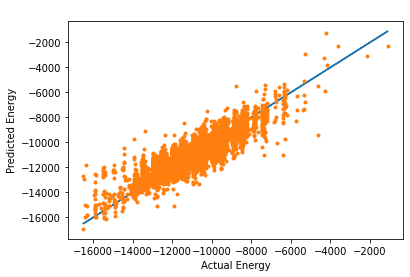
\includegraphics[width=.8\linewidth]{qm9-nn-result.png}
      \caption{QM9 dataset classical neural network approach}
      \label{fig:sfig1}
    \end{subfigure}%
    \begin{subfigure}{.5\textwidth}
      \centering
      \captionsetup{justification=centering}
      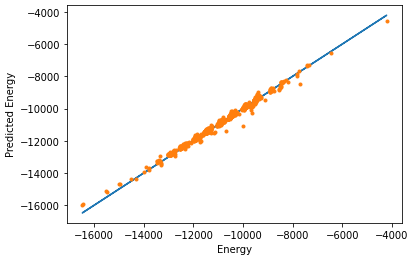
\includegraphics[width=.8\linewidth]{qm9-gnn.png}
      \caption{QM9 dataset graph-based neural network approach}
      \label{fig:sfig2}
    \end{subfigure}
    \begin{subfigure}{.5\textwidth}
        \centering
        \captionsetup{justification=centering}
        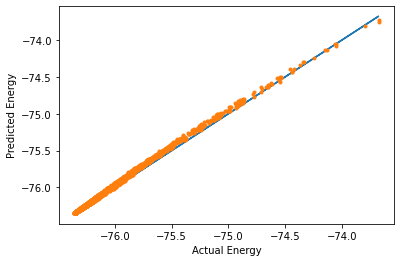
\includegraphics[width=.8\linewidth]{water-nn.png}
        \caption{Water dataset classical neural network approach}
        \label{fig:sfig3}
      \end{subfigure}
      \begin{subfigure}{.5\textwidth}
        \captionsetup{justification=centering}
        \centering
        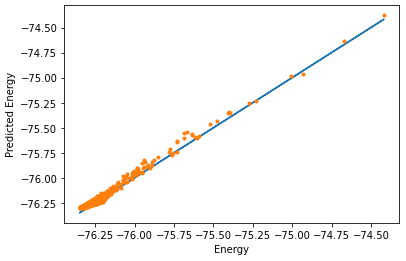
\includegraphics[width=.8\linewidth]{water-gnn.png}
        \caption{Water dataset graph-based neural network approach}
        \label{fig:sfig4}
      \end{subfigure}
    \caption{Comparison of actual and predicted energy from the different datasets}
    \label{fig:plotsofresults}
    \end{figure}

To summarize the evaluation, it can be said that the use of a GCN architecture is particularly useful when the dataset is complex and contains different atoms and chemical compounds, as is the case with the QM9 dataset. In contrast, the use of a basic neural network architecture is recommended for rather simple datasets, such as the water dataset used previously. \\

During the last phase of the CRISP-DM process, the developed and evaluated GCN can be deployed and make use of the knowledge gained. In the course of this paper, the developed GCN is a prototype and will be further used for the comparison to other machine learning models in the context of potential energy surface prediction. 

\section{Conclusion}
Overall, the conducted research process has proven to be suitable for the literature review, followed by the development of the GCN for molecular property prediction. In this chapter, the results are summarized and critically reflected upon, and future research potential is identified. 

\subsection{Summary}

Within the scope of the literature review, in total 11 different architectures or approaches for the implementation of GNNs could be identified and further categorized. Furthermore, an overview over the differences between the identified approaches and architectures was given. Utilizing the information gained in the scope of the literature review, the convolutional approach of a GNN was used for the development of a GNN that predicts the potential energy surface of a molecule. By using the in the discipline of computational chemistry frequently used QM9 dataset for the development of the model, the results can be adapted to other datasets that contain different information, e.g. in form of other molecules.  

\subsection{Critical Reflection}
As mentioned before, the research methodology was suitable for analyzing the findable literature and for the prototypical implementation of the GNN. However, this work also has its limitations. Further approaches or architectures of GNNs could have been investigated to be used for the prediction of potential energy surfaces. By doing so, a comparison between the results, e.g. with measured performance metrics, could have taken place. In addition, the developed GNN could have been tested with other datasets than the QM9 dataset, to be able to evaluate its general validity. These aspects might have identified important requirements that are not included in the current iteration of the prototypical GNN.

\subsection{Outlook}

The insights in gained in this paper provide a starting point for future research. The QM9 dataset, that was used in this paper, provides quantum chemical properties at DFT level. Besides, the prediction of potential energy surfaces and other relevant properties proceeds at the molecular and atomic level. The advancing development of quantum computers raises the question, if machine learning models like GNNs that compute quantum properties like potential energy surfaces can be realized on quantum computers. While there already exist first approaches of quantum graph neural networks in the literature \cite{verdon_quantum_2019,beer_quantum_2021,ai_decompositional_2023}, the results of the literature review and the developed GNN in this paper serve as a starting point for a further investigation in the field of quantum graph neural networks. 

\chapter{Quantum Graph Neural Networks for Molecular Property Prediction}

\section*{Abstract}

Hydrogen research, particularly in the fields of energy storage and catalysis, hinges on a deep understanding of molecular interactions and properties. The surface area of molecules is a crucial parameter influencing hydrogen adsorption and catalytic efficiency. Traditional computational methods for predicting molecular surface areas, while effective, face challenges in terms of computational complexity and accuracy when dealing with large and complex molecular structures. The accurate prediction of molecular surface area is paramount in optimizing hydrogen storage and catalysis processes. Conventional computational models, primarily based on classical algorithms, struggle with the vast complexity and quantum nature of molecular systems. This gap necessitates a novel approach that can handle the quantum mechanical properties inherent in molecules more naturally and efficiently.

\textit{\textbf{Keywords:} quantum machine learning, quantum graph neural networks, hydrogen research, potential energy surface prediction}

\section{Introduction}
\label{sec:introduction}

In view of the steadily advancing climate change, efforts to reduce environmental pollution are
increasingly coming into focus both in the public eye and within the scientific community \cite{amin_hydrogen_2022}.
This includes the search for scalable and cost-effective renewable energy storage solutions, which
is essential to meet the world's growing energy demand while mitigating climate change \cite{kilkis_research_2019}. The
conversion of electricity to hydrogen, as well as the reverse combustion process, can play an
important role here \cite{amin_hydrogen_2022}. Therefore, new materials are constantly being investigated to enable
catalytic processes in the field of hydrogen production to run efficiently \cite{chen_waste-derived_2023}. Machine learning
methods are already being used to simulate and calculate catalytic properties. In particular, graph
neural networks (GNN) are proving to be especially promising here \cite{tran_open_2023, bronstein2017geometric}. Since the prediction of potential areas and other relevant properties takes place at the molecular and atomic level, the use of quantum computing or quantum machine learning is an interesting direction of research in the field of molecular properties. There is currently a growing interest in exploring the application of quantum computers in various domains \cite{valdez2023review}. The results of Tychola et al., which are also shown in Figure \ref{img:tychola}, show that the number of publications in the field of quantum machine learning has drastically increased since 2017 and that German research is also making a significant contribution to this \cite{Tychola_Kalampokas_Papakostas_2023}.

\begin{figure}[h!]
    \begin{subfigure}{.5\textwidth}
     \captionsetup{justification=centering}
      \centering
      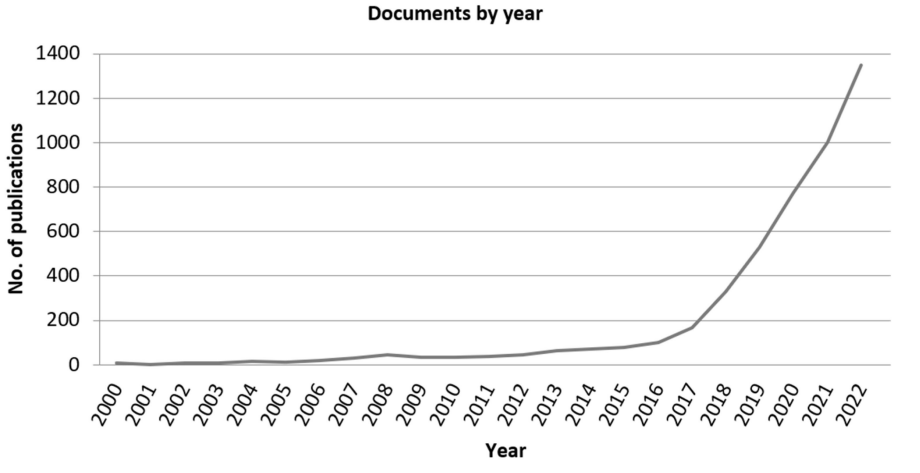
\includegraphics[width=.8\linewidth]{QML-Documents.png}
      \caption{Number of documents released per year in the field of QML}
      \label{fig:sfig1}
    \end{subfigure}%
    \begin{subfigure}{.5\textwidth}
      \centering
      \captionsetup{justification=centering}
      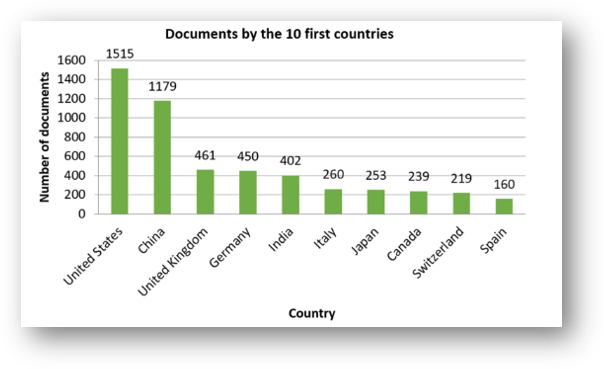
\includegraphics[width=.8\linewidth]{QML-countries..png}
      \caption{Number of documents released per country in the field of QML}
      \label{fig:sfig2}
    \end{subfigure}
    \caption[Results of QML-Literature-Overview from Tychola et al. 2023 (excerpt)]{\label{img:tychola} Results of QML-Literature-Overview from Tychola et al. 2023 \cite{Tychola_Kalampokas_Papakostas_2023} (excerpt)}
    \end{figure}

The literature also shows that first approaches to realize GNNs on quantum computers already exist \cite{verdon_quantum_2019, beer_quantum_2021,ai_decompositional_2023,zheng2021quantum,ryu2023quantum}. The resulting combination of quantum machine learning and graph neural network models is called Quantum Graph Neural Networks (QGNNs). However, the specific application of predicting molecular properties by using QGNNs, particularly in hydrogen research, remains underexplored in the literature. This provides an opportunity to bridge the gap between quantum computing and molecular science in the context of hydrogen storage and catalysis. \\
    
In order to solve the presented problem, the following research question and sub-questions are created: 

\begin{center}
    \textit{"How can a Quantum Graph Neural Network for the prediction of molecular properties be developed?"} \\
\end{center}
Q1: \textit{How do Quantum Graph Neural Networks work?} \\
Q2: \textit{How must molecular data be processed to be used with a quantum computer?} \\
Q2: \textit{How does the performance compare to classical Graph Neural Networks?} \\

The goal of this paper is to develop an understanding of QGNNs and how they work. Besides, in the scope of this paper, an understanding of the prediction of potential energy is created. Based on this procedure, the analysis of different foundation papers will show how a QGNN can be developed. In summary, to answer the developed research question and sub-questions, the following artifacts will be created as part of the research: 

\begin{itemize}
    \item foundation paper analysis of different papers in the context of quantum graph neural networks
    \item based on the foundation paper analysis: requirements analysis to identify the requirements for the development of a quantum graph neural network that is able to predict molecular properties 
    \item attempt to develop a quantum graph neural network based on the conducted requirement analysis
\end{itemize}  

The structure of this paper is as followed: first, the scientific foundations and theoretical background are discussed. Then the research methodology is presented in detail. Based on this, the findings and their results are presented and then discussed. Finally, a conclusion and discussion of the results is provided, as well as an overview of possible research topics based on this work.   

\section{Theoretical Background}
\subsection{Quantum Computing}
In order to understand the fundamentals of quantum computing, it is first necessary to explain the basic building blocks of quantum computing. These are also known as quantum bits, quantum gates and quantum circuits, and are explained in the following. In quantum computing, quantum bits, or qubits, are the basic units of information. Unlike classical bits, which can only take the states 0 or 1, qubits operate according to the principles of quantum mechanics, which allows them to take both states simultaneously. \cite{claudino2022basics} Quantum gates are the building blocks for quantum circuits and perform operations on qubits. They are the analogue of logic gates in classical computer science, but with the difference that quantum gates perform continuous transformations, also known as unitary transformations, which change the superposition states of the qubits. An example of single quantum gates are Pauli rotation gates, which are displayed in Table \ref{tab:pauligates}. These are applied by extracting the exponentials of the Pauli operator.

\begin{table}[h!]
    \centering
    \captionsetup{justification=centering}
    \begin{tabular}{ccc}
    \hline
    \textbf{Gate} & \textbf{Matrix Representation} \\ 
    \hline
    $R_x$ gate & $\begin{pmatrix} \cos\frac{\theta}{2} & -i\sin\frac{\theta}{2} \\ -i\sin\frac{\theta}{2} & \cos\frac{\theta}{2} \end{pmatrix}$ \\ 
    $R_y$ gate & $\begin{pmatrix} \cos\frac{\theta}{2} & -\sin\frac{\theta}{2} \\ \sin\frac{\theta}{2} & \cos\frac{\theta}{2} \end{pmatrix}$ \\ 
    $R_z$ gate & $\begin{pmatrix} e^{-i\frac{\theta}{2}} & 0 \\ 0 & e^{i\frac{\theta}{2}} \end{pmatrix}$ \\ 
    \hline
    \end{tabular}
    \caption[Pauli-rotation gates according to Zheng et al. 2021]{\label{tab:pauligates} Pauli-rotation gates according to Zheng et al. 2021 \cite{zheng2021quantum}}
\end{table}

There are also two-bit gates, which perform operations on two qubits and thus logically link them together. One example of this is the CNOT gate, which is used frequently in the field of quantum computing. \cite{zheng2021quantum} Quantum circuits are a combination of the previously introduced quantum gates and qubits. This is a specific sequence of quantum gates that are applied to a specific number of qubits in order to perform complex calculations. A quantum circuit is always designed for a specific application. This enables a variety of specific applications such as the simulation of molecular interactions. \cite{claudino2022basics} 

Following the basic building blocks of quantum computing, entanglement and superposition are important elements of quantum computing and enable a new form of information processing. Firstly, entanglement means that the state of one qubit can directly influence the state of another, regardless of spatial separation. Superposition allows a qubit to be in a superposition of different states, which enables parallel processing of several calculations in a single step. This phenomenon enables, among other things, the acceleration of optimization problems in (quantum) machine learning calculations, such as the improvement of pattern recognition algorithms. This results in accelerated computation in a variety of applications, such as the prediction of molecular properties. \cite{dunjko2017machine} 

Quantum data encoding describes how information can be processed in such a way that it can be used on a quantum computer. In summary, there are four different data encoding strategies: basic encoding, in which classical bits are mapped to qubits using the basic states 0 and 1, superposition encoding, in which qubits are placed in a superposition of classical states, angle encoding, in which classical information is encoded as relative phases between different quantum states, and finally amplitude encoding, in which classical information is translated into the amplitudes of the quantum states \cite{rath2023quantum}. Amplitude encoding is  often used when feature maps are used. These feature maps describe functions that automatically translate classical information into the complex amplitudes of a quantum state. Feature maps are frequently used in the field of quantum machine learning (QML) in particular. \cite{schuld2015introduction} For example, IBM's quantum computing library Qiskit contains usage ready feature maps \cite{ZZFeatureMap}. This data encoding process is a key step for the application of quantum computers, as it makes it possible to apply the parallel computing capacities of quantum computers to real-world data \cite{rath2023quantum}. Essentially, encoding translates classical data into the language of quantum physics, allowing quantum algorithms to be applied to problems like the prediction of molecular properties.

The principle of quantum processing describes the processing of encoded data using quantum states and quantum operations. In the field of QML, various quantum algorithms already exist, such as quantum support vector machines and quantum neural networks, which make the principles of classical algorithms usable for quantum computers \cite{biamonte2017quantum}. Together with the encoded classical data into the quantum state, these algorithms can e.g. solve regression and classification tasks by utilizing the parallel nature and superposition capability of quantum computers. 

The overarching goal of quantum computing is to achieve the "quantum advantage". This term refers to the superiority of quantum computing over classical computing in terms of solving complex problems in various fields, such as machine learning \cite{daley2022practical}. In the future, quantum hardware will be able to solve practical problems that even supercomputers cannot solve.

%\subsection{Quantum Graph Neural Networks}
\subsection{Potential Energy Prediction}
The potential energy surface (PES), in the context of molecules and atoms, describes the energy of a molecule in regard to certain parameters, e.g. to the position of its atoms.    
Predicting the potential energy surface of atoms is a task in computational chemistry and materials science. It gives information about the stability and properties of molecules and materials \cite{liu_computational_2023}. This is helpful when to decide whether materials can be used to enable efficient catalytic processes in the field of hydrogen production \cite{chen_waste-derived_2023}. 

\section{Research Methodology}

First, the given problem of constructing QGNNs for the prediction of molecular properties was investigated. For this purpose, an initial investigation of the literature took place and the topic was explored. This is followed by the definitions of the research questions as well as the sub-questions and the delineation of the research topic. \\

\begin{figure}[h!]
    \centering
    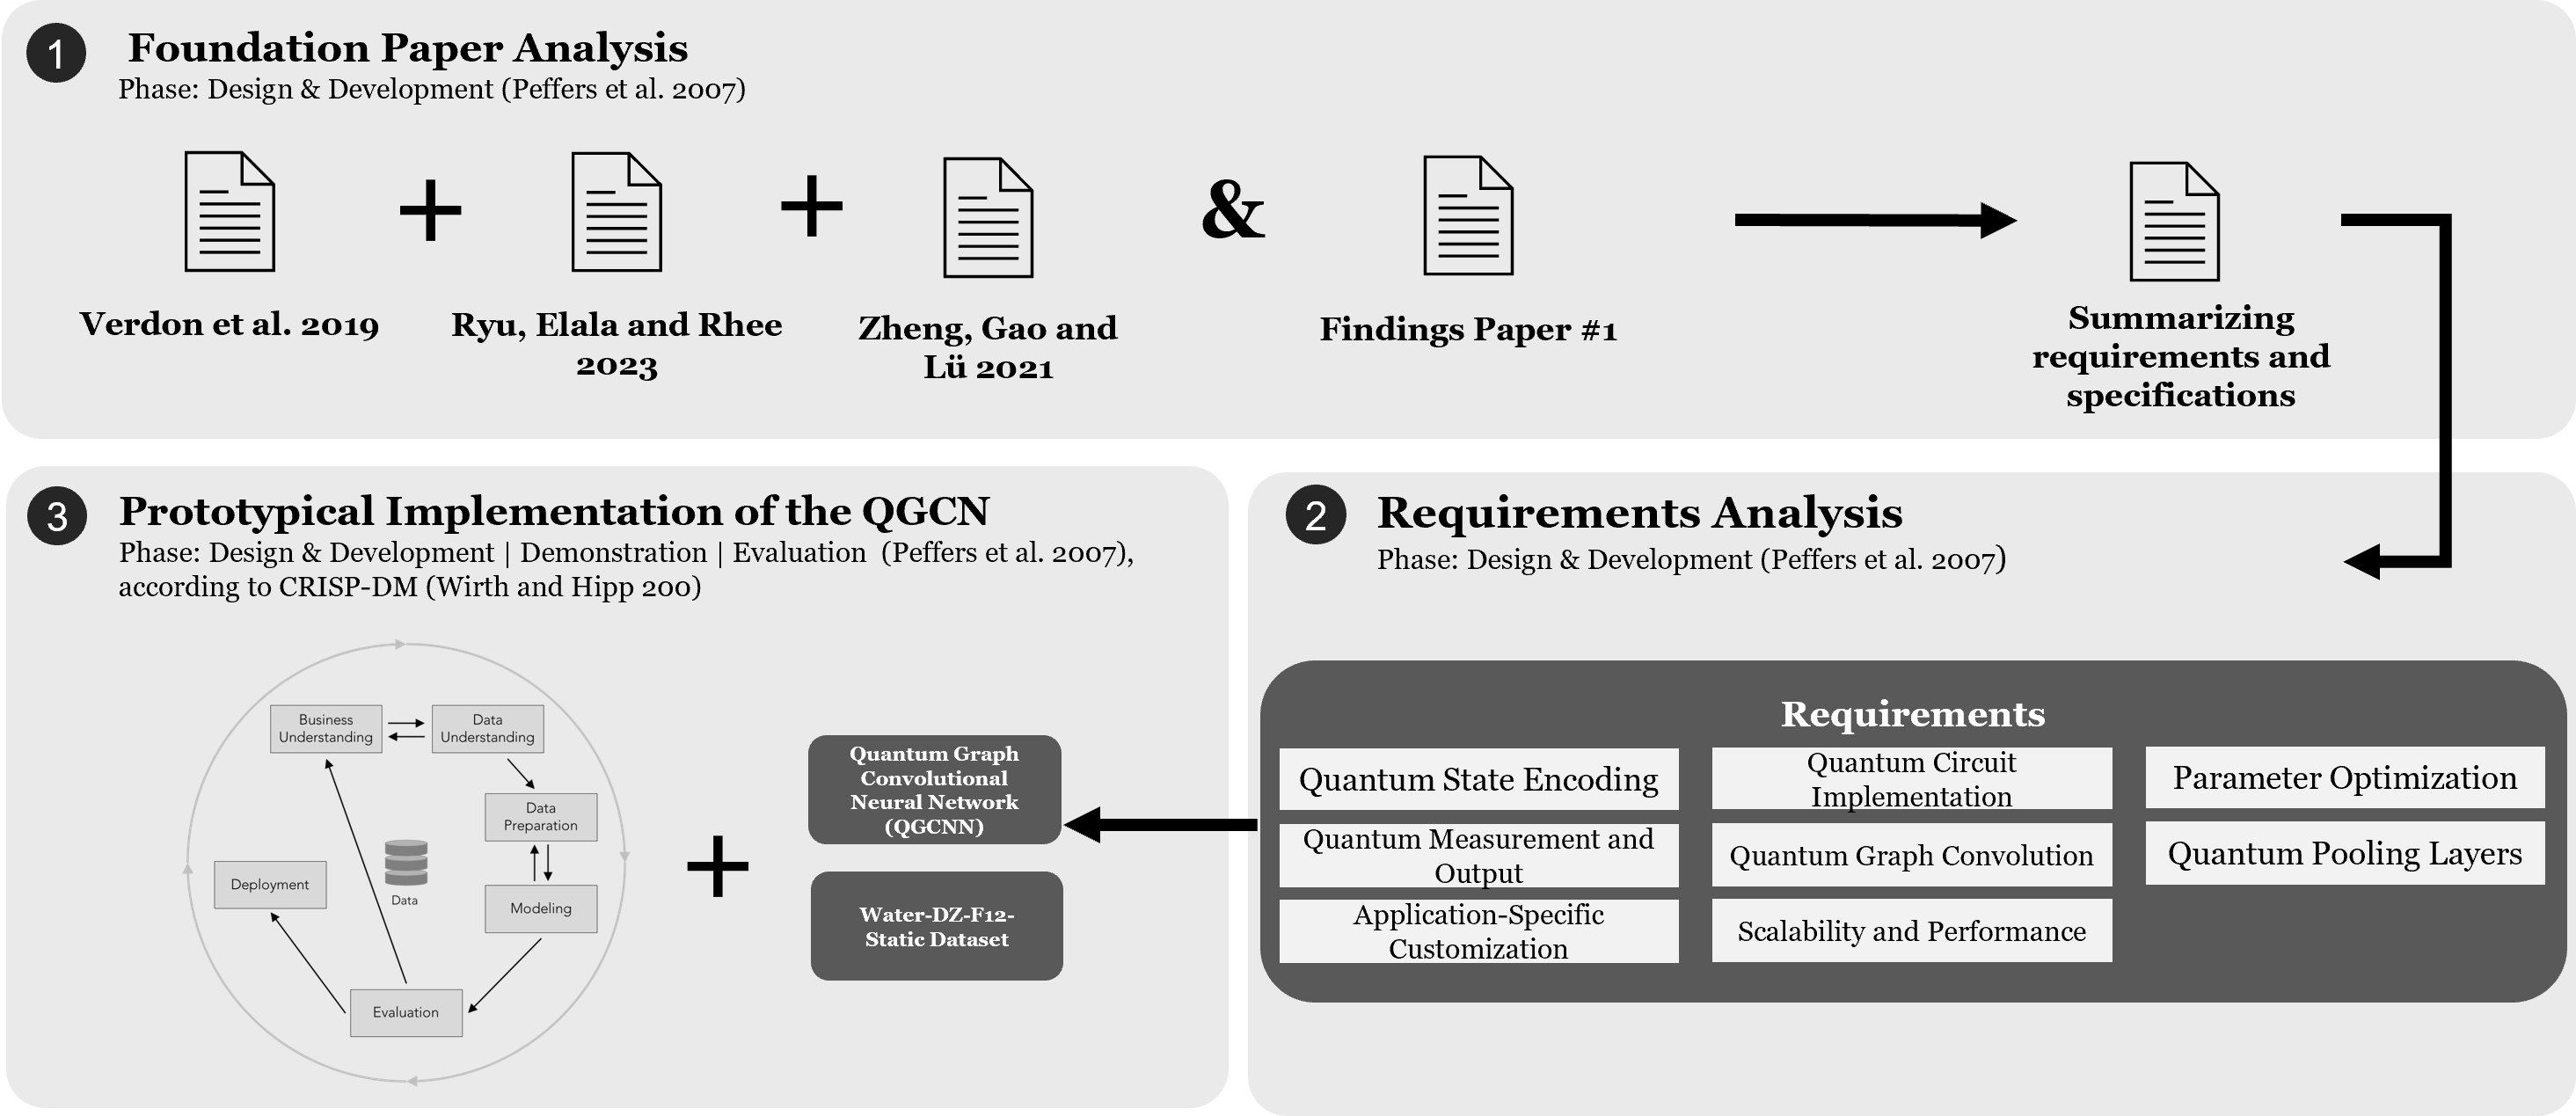
\includegraphics[width=\textwidth]{05_paper02RM.png}
    \caption[Overview of the conducted research process]{\label{img:paper02rm}{Overview of the conducted research process}}
    \end{figure} 

Three foundation papers were then analyzed to investigate different approaches to the development of QGNNs and to identify a possible approach to the development of a QGNN for the prediction of molecular properties. Similar to the results of the first paper of this thesis and the results of the foundation paper analysis, requirements for a Quantum Graph Convolutional Neural Networks (QGCN) to be developed are defined. Using these requirements, this paper will attempt to develop a prototpyical QGCN. For a better structure and traceability of the procedure, the exact research process is shown in Figure \ref{img:paper02rm} on the previous page, which is described in detail in the following section. \\

The \textbf{first step} was to analyze the foundation papers. The papers by Verdon et al. \cite{verdon_quantum_2019}, Zheng, Gao and Lü \cite{zheng2021quantum} and the paper by Ryu, Elala and Rhee \cite{ryu2023quantum} were used. Since the literature on QGNNs is limited to a very small number of papers, a structured literature analysis is not useful in this case. Accordingly, various literature databases were searched for literature on QGNNs and the papers most relevant to the topic of this thesis were selected for the foundation paper analysis. The results of the analysis of these three papers were combined with the results of the first paper of this thesis and summarized for the next step of the conducted research process. \\

In the \textbf{second step}, a requirements analysis was carried out based on the results of the foundation paper analysis. Based on the results of the first paper of this thesis, the goal was to implement a QGCN. Therefore, a total of 8 different requirements were identified for the QGCN to be developed. The results of this requirements analysis are discussed in more detail in Section \ref{subsec:requirements}. \\

The \textbf{third step} covers the prototypical implementation of the QGCN for the prediction of molecular properties. Based on the previously identified requirements, an attempt was made to implement a QGCN capable of predicting the potential energy surface using the water data set mentioned in the first paper of this thesis. Similar to the first paper, the implementation followed the structured procedure of CRISP-DM \cite{wirth2000crisp} and is explained in Section \ref{subsec:qgnndevelopment} of this thesis. Although the QGCN could not be implemented completely successfully, the development still provides interesting insights and further work can be based on the findings of this paper.

\section{Findings}
In this section, the results and findings are presented and discussed in detail. First, the analyzed foundation papers are summarized and the relevant information is extracted. Afterwards, the identified requirements given from the analysis of the foundation papers are explained in detail in the requirement analysis. As the QGCN could not be fully implemented successfully, the development of a Quantum Convolutional Neural Network (QCNN) capable of predicting potential energy surface and forming the starting point for a QGCN is demonstrated. In a final step, the challenges of implementing the QGCN are documented.

\subsection{Foundation Papers}
This section briefly summarizes all foundation papers that were read and used for the requirement analysis as shown in the first step of the conducted research process in the previous section. \\

In the paper by Verdon et al. from 2019 \cite{verdon_quantum_2019}, the authors discuss the development of Quantum Graph Neural Networks. These are quantum computing models for processing information that is represented in graph structures. The authors investigate the development of two architectures (also called ansatze in the field of quantum computing) for QGNNs: Quantum Graph Convolutional Neural Networks and Quantum Graph Recurrent Neural Networks (QGRNNs). These architectures are designed to use quantum mechanical properties to efficiently perform computational tasks on graph-structured data. Therefore, at first, the quantum circuits and algorithms on which the QGNNs ansatze are based are presented. The authors show how QGNNs can be applied to different information processing tasks, such as learning quantum hamiltonian dynamics or the execution of a graph classification task. By performing various experiments, the authors validate the proposed ansatze for the QGNNs. The performance of QGNNs in solving graph-theoretic problems is demonstrated by running simulations in comparison with classical graph neural networks. The results of these simulations show the potential of QGNNs to advance graph-based machine learning in the field of quantum computing by providing an efficient way to solve graph-theoretic problems. \\

The development and application of Quantum Graph Neural Networks for predicting the properties of molecules and materials is explored in the paper of Ryu, Elala and Rhee from 2023 \cite{ryu2023quantum}. This contribution is therefore closest to the topic of this thesis. The focus of this paper is on the prediction of the energy gap between the highest occupied and the lowest unoccupied molecular orbitals (HOMO-LUMO) of small organic molecules.  The authors present an ansatz that they call the Equivariantly Diagonalisable Unitary Quantum Graph Circuit (EDU-QGC). This ansatz is specifically designed to encode discrete bond features and optimizing the embedding process within quantum circuits, ensuring a more efficient representation of molecular structures. For the data encoding, the authors use the method of angle encoding with $R_y$ or $R_z$ gates, which is a common strategy when encoding data into the quantum state. In the EDU-QGC circuit design, the molecular bonds are represented as single or double link bonds, depending on the structure of the molecule. The authors evaluate two different readout functions: a local readout function that reads from node-local terms and a global readout functions that reads out the information given on all nodes in the graph.
In the course of experimental testing and evaluation of the developed model, the QM9-Dataset has been used by the authors, divided into 10,000 training and 1000 testing samples.  The results of the experiments conducted demonstrate the effectiveness of the QGNN model and show that it can achieve lower test losses in predicting the HOMO-LUMO gap than classical neural graph network models with a comparable number of trainable parameters. In addition, the QGNN model converges faster in the training phase, thus indicating a more efficient learning process. The authors make no general claim to the so-called "quantum advantage", but the results suggest that quantum-enhanced graph neural networks are  a promising area of research for the field of materials science and molecular chemistry. \\

The last paper describes the work of Zheng, Gao and Lü from 2021 \cite{zheng2021quantum}. In the paper, the authors describe the development of a Quantum Graph Convolutional Neural Network, which was developed for classification tasks at the graph level. They proceed according to the following steps: first, the graph data is en coded into the quantum state using amplitude encoding, next universal parameter-based gates circuits are used for the construction of the QGCN by using the amplitude encoded graph data and last, the learning ability of the QGCN is tested by training on a quantum circuit using the MNIST dataset for classification benchmarking. Accordingly, the authors develop a quantum analogue of classical graph convolutional layers that allows quantum circuits to encode graph information and perform convolutional and pooling operations. This QGCN ansatz processes graphs by encoding node features and structural information such as the connections between the nodes into quantum states, and then applying parametrized quantum gates to simulate convolutional and pooling operations. According to the authors, this ansatz makes it possible to capture patterns and relations between nodes within the graph structure. To test the proposed QGCN ansatz, the authors use the MNIST dataset in their experiments, which contains handwritten digits and is often used for benchmarking classification tasks. The results of the experiments show that the developed QGCN ansatz achieves a high accuracy of 0.90 (one convolutional layer and one pooling layer) or 0.91 (two convolutional layers and one pooling layer). These results demonstrate that graph data can be efficiently processed using quantum computing and accurate predictions can be made.

\subsection{Requirement Analysis}

Following the summary of the foundation paper, this chapter presents the requirements identified in the foundation paper. The Figure \ref{img:requirements} shows an overview of the eight requirements. These are considered and explained in detail below

\begin{figure}[h!]
    \centering
    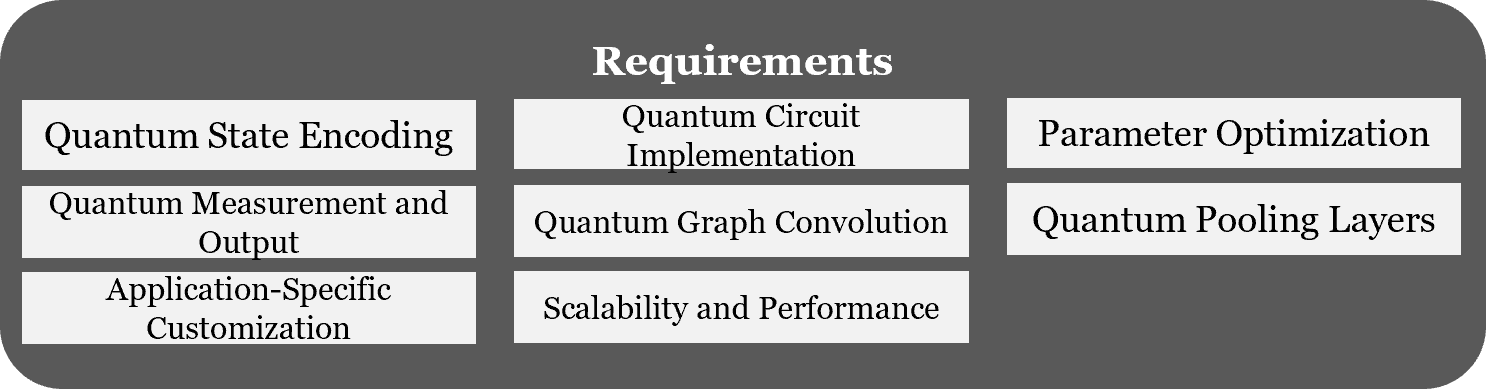
\includegraphics[width=\textwidth]{requirements.png}
    \caption[Identified requirements from the requirement analysis]{\label{img:requirements}{Identified requirements from the requirement analysis}}
    \end{figure} 

The first requirement describes quantum state coding, i.e. the encoding of classical data into quantum states. To develop a QGCN, the graph structures must be converted into quantum states. This involves encoding the node and edge information onto the qubits. Two different strategies were used in the foundation papers: amplitude encoding \cite{zheng2021quantum} and angle encoding \cite{ryu2023quantum}. The best encoding strategy depends on the underlying use case and must be tested during implementation. In the case of predicting potential energy surfaces for molecules, the atoms need to be coded with their coordinates and chemical bonds as nodes, and the regression target needs to be linked to the coordinates of the molecules. \\

The second requirement is the implementation of the quantum circuit and thus the structure of the implemented quantum circuits for data processing. Hereby, the number of qubits plays a major role. For data sets with a relatively small number of features, it is possible to map one feature onto one qubit. For graph-based data, however, it is necessary to use several qubits to map the relationships between the atoms of a molecule. In this way, the qubits are manipulated and the weights within the molecules are represented based on the atomic coordinates and chemical bonds. The design of the circuits has a major impact on the performance and accuracy of a QGCN, i.e. its ability to learn from graphically structured data and make predictions. \\

Another requirement for the QGCN to be developed is the parameter optimization. In QML or quantum circuits, parameters are used to learn and store relationships in data sets to enable later predictions. Parameter optimization is necessary to minimize the loss function when training a QGCN and to obtain accurate prediction results. This is done in a similar way to the parameters used to train classical neural networks. To learn the correlations in the data, the number of parameters should always be greater than the number of features used. \\

Quantum measurement and output comprises a further requirement resulting from the analysis of the foundation papers. This refers to the way in which measurements are performed during calculations in quantum circuits. In the field of QML, measurements are the probability distributions that result from the calculations within the quantum circuits. So-called observables are used for this purpose. The challenge is to recognize where and with how many qubits measurements should be made. For QGCNs, quantum measurement is limited to the measurement of single or double qubits after pooling operations have been carried out. In the context of QGCNs, the quantum information is translated into a form that can be used for further tasks, such as the classification of graphs. \\

The following two requirements can be summarized and describe the architecture of the QGCN in addition to data encoding and quantum measurement. These are the quantum graph convolution and quantum pooling layer requirements. Quantum graph convolution is analogous to classical convolutional operations on graph data. Parameterized quantum circuits are used to compute local and global neighborhood structures between nodes and to learn feature weights. In this way, the QGCN can recognize the connectivity and relationship patterns within a graph.

The requirement for quantum pooling layers refers to the introduction of the pooling mechanism, which is also used in classical convolutional neural networks. The pooling mechanism aims to reduce the dimensions of the feature space and thus the computational cost, while preserving the important features. In quantum pooling, the number of qubits in the QGCN is reduced by stringing together different convolutional and pooling layers to enable efficient measurement operations on one or two qubits during the training of the QGCN. \\

The application-specific adaptation of a QGCN describes the second last requirement during the development a QGCN. When designing quantum circuits, they must always be designed and implemented taking into account the underlying (graph) data and are therefore application dependent. In the case of the QGCN for predicting molecular properties, this concerns the number of qubits, the structure of the quantum circuits, the number of parameters in the quantum circuits and the number or arrangement of the convolutional and pooling layers. This ensures that the QGCN can learn effectively from the properties of the dataset and the underlying use case. This is closely related to the last requirement, scalability and performance. As quantum hardware in particular is constantly evolving, the QGCN needs to be scalable to continue to use qubits and quantum circuits to achieve improved performance and efficient use of available computational resources. This step should also ensure that data sets of different sizes can be used in the field of molecular property prediction.

\label{subsec:requirements}
\subsection{Development of the QCNN}
\label{subsec:qgnndevelopment}

After gaining insight into the requirements of a QGCN, it was attempted to develop a QGCN for the prediction of molecular properties. It was possible to develop a QCNN consisting of a convolutional layer and a pooling layer. The development of the QCNN in this paper is based on the QCNN of the Qiskit ecosystem \cite{qcnn}. However, it was not possible to fully implement the processing and interpretation of the graphs. This paper therefore documents the development of the QCNN, which can be used as the basis for a QGCN. This QCNN was trained with a data set containing only water molecules, similar to the first paper in this thesis. The development of the GCN was based on the established CRISP-DM process \cite{wirth2000crisp}, which is explained step by step below. \\

The first phase of the CRISP-DM process refers to business understanding and is essentially the same as the introduction from Chapter \ref{sec:introduction}. For reasons of focus, this phase is therefore not listed separately again. However, in the second phase of the process, data understanding, the aim is to provide an insight into the given data set. As already mentioned, a data set consisting of approx. 36,000 water molecules is used.  This data set contains molecules consisting of oxygen and hydrogen atoms, which have different atomic coordinates. The relevant target variable is also contained in the data set and describes the potential energy surface of the atom. \\

In the next step, the dataset will be prepared to be able to train the developed QCNN. The data preparation includes at first the extraction of all relevant information from the dataset, which is in this case the atoms, the cartesian coordinates of the atoms which are the features and the regression target variable. For better results off the model predictions, the target variables are normalized with the help of their mean and standard deviation. Additionally, the features are normalized between a range of 0 and 1 which is an important step before encoding data into the quantum state. \\



\begin{table}[h!]
    \centering
    \captionsetup{justification=centering}
    \resizebox{\textwidth}{!}{
        \setlength{\tabcolsep}{1.5em}
        {\renewcommand{\arraystretch}{1.5}% for the vertical padding
            \begin{tabular}{p{7cm} l l}
                \hline
                 \textbf{Parameter} & \textbf{Amplitude Encoding} & \textbf{Angle Encoding} \\
                 \hline
                   Training time &  3 min 52.3s & 3 min 27.8s  \\
                   Mean Squared Error (MSE) & 0.2359 & 0.2150 \\
                   Root Mean Squared Error (RMSE) & 0.0667 & 0.0585 \\
                   Train data accuracy ($R^2$) &  85.87\% & 89.27\%  \\
                   Test data accuracy ($R^2$) &  85.65\% & 88.98\%  \\
                   \hline
               \end{tabular}
           }
       }
       \caption[Comparison of performance metrics of the developed model with different data encoding strategies]{\label{tab:paper02performancecomparison} Comparison of performance metrics of the developed model with different data encoding strategies}
\end{table}

\subsection{Challenges during the development}

\section{Conclusion}
Although the primary research question could only be answered theoretically, the results show a structured approach to the development of a QGCN and form a solid basis for further work. Accordingly, the research process that was carried out proved to be suitable for the answering of the underlying research questions. This chapter summarizes and critically reflects on the results and identifies future research potential.

\subsection{Summary}
During the analysis of the foundation papers, three papers were identified that provide information on the development of QGNNs. Based on these papers, a total of 8 different requirements for the implementation of a QGCN that has a similar architecture to the developed model from the first paper of this thesis could be identified. These requirements were explained individually. This approach leads to a theoretical answer to the research question of this paper. Using the information from the foundation papers and the requirements, an attempt was made to develop a QGCN that predicts the potential energy surface of molecules. As the QGCN could not be implemented completely successfully, the development was documented using a QCNN that also predicts molecular properties. Nevertheless, the research process and its results in terms of the requirements and the development of the QCNN provide valuable insights into the development of the QGCN and form a solid basis for further work. 

\subsection{Critical Reflection}

\subsection{Outlook}

\chapter{Overall Conclusion}
\label{global:conlusion}
\section{Summary and conclusion}
This thesis contributes research in the field of graph neural networks and quantum computing as well as the prediction of molecular properties. First, classical graph-based deep learning methods from the existing literature are analyzed and prototypically implemented. Later, these findings will be combined with quantum computing principles to investigate a problem from computational chemistry and materials science. The focus is on hydrogen compounds and their potential energy surfaces, which are an indicator for catalytic processes in hydrogen production. \\ 

This cumulative thesis is divided into two papers, each describing the development and evaluation of models for the given problem. In the first paper, a classical graph-based convolutional neural network model is implemented and tested using the QM9 dataset and a simpler water dataset, each describing a collection of molecules with quantum chemical properties. This model serves as a fundamental step in demonstrating the effectiveness of GNN architectures in capturing the relationships within molecular structures and enabling the prediction of molecular properties. The second paper provides insights into the field of quantum computing and attempts to extend the convolutional GNN architecture to its quantum counterpart, a Quantum Graph Neural Network, using the limited literature available.
In order to summarize the findings of this thesis and its contribution to the field of research, the following artifacts were created during the research process:

\begin{itemize}
    \item literature review of different graph neural network architectures
    \item prototypical implementation of a graph neural network for the potential energy prediction
    \item baseline neural networks for the comparison to graph-based models with different datasets
    \item foundation paper analysis of different papers in the context of quantum graph neural networks
    \item based on the foundation paper analysis: requirements analysis to identify the requirements for the development of a quantum graph neural network that is able to predict molecular properties 
    \item attempt to develop a quantum graph neural network based on the conducted requirement analysis
    \item implementation of a quantum convolutional neural network architecture as a basis for further development on quantum graph-based models
\end{itemize} 

Although the realization of a QGNN could not be fully implemented due to various challenges, such as the limited literature on the integration of quantum computing and graph-based machine learning, a prototype quantum convolutional neural network architecture was successfully developed. This prototype represents an important step towards utilizing the potential of quantum computing for graph-based information processing at the molecular and atomic level. As shown, several artifacts were created as part of this work. Thus, this work contributes to the field of hydrogen research and the prediction of molecular properties by combining the theoretical investigation of the problem at hand with the practical development and evaluation of models not only on classical computers but also on quantum computers. \\

In summary, this work not only highlights the potential synergies between quantum computers and neural networks for comprehensive molecular predictions, but also provides a foundation and path for future research. Overall, the development of complex deep learning algorithms to utilize quantum hardware is still at an early stage. Further advances in quantum computing and quantum machine learning will be necessary to fully exploit the potential of e.g. quantum graph-based neural networks in computational chemistry and thus harness the power of quantum computing and achieve the quantum advantage status in the future. 


%\newpage
%\section{Critical Reflection}
%\newpage
%\section{Outlook}
%\newpage


%============ Literature ================%
\pagestyle{plain}
\renewcommand*{\chapterpagestyle}{plain}
\clearpairofpagestyles
\cfoot[\pagemark]{\pagemark}
\pagenumbering{Roman}
\setcounter{page}{6}
\printbibliography

%\phantomsection
\addcontentsline{toc}{chapter}{Appendix}
\chapter*{Appendix}
\appendix
\section*{A. Model comparison with QM9 dataset}
\label{appendix:qm9modelcomparison}


\newpage

\section*{B. Model comparison with water dataset}
\label{appendix:watermodelcomparison }

%\renewcommand\appendixtocname{Anhang}
%\renewcommand\appendixpagename{Anhang}
%\begin{appendices}
%\end{appendices}

\end{document}
